% Importado desde: 2026-03-28_Desdoblamiento_Controlado_Dirac_a_Weyl_en_3D.tex
\chapter{Derivacion Pedagogica: --- desdoblamiento controlado de Dirac a Weyl en \(3D\)}
\label{ch:desdoblamiento-dirac-a-weyl-3d}






% verified-by: validators/desdoblamiento.py::test_squared_decomposition
% verified-by: validators/desdoblamiento.py::test_upper_weyl_node
% verified-by: validators/desdoblamiento.py::test_lower_weyl_node
% verified-by: validators/desdoblamiento.py::test_node_separation

\section{Objetivo}
En el capitulo anterior conseguimos algo muy importante: una dinamica discreta de tipo Wilson--Dirac en la que un solo subsector queda ligero, mientras los dobladores permanecen pesados.

Ahora damos el siguiente paso delicado:
\begin{displayquote}
\textbf{introducir una perturbacion concreta que desdoble ese sector Dirac ligero en un par de nodos Weyl, sin volver a contaminar la teoria infrarroja con los dobladores pesados.}
\end{displayquote}

Este paso tiene dos partes distintas:
\begin{enumerate}[label=\arabic*.]
    \item mostrar como un cono de Dirac ligero se separa en dos nodos Weyl;
    \item justificar que ese desdoblamiento ocurre solo en el subsector deseado.
\end{enumerate}

Vamos a hacerlo con un modelo muy concreto y con una cuenta completamente controlable.

\section{La idea fisica antes de escribir formulas}
Un fermion de Dirac en \(3D\) puede verse como la superposicion de dos sectores de quiralidad opuesta. Para separarlos necesitamos una perturbacion que:
\begin{enumerate}[label=\arabic*.]
    \item distinga una direccion espacial;
    \item distinga los dos sectores quirales;
    \item rompa la simetria que mantenia ambos sectores pegados en el mismo punto del espacio recíproco.
\end{enumerate}

La perturbacion mas pedagogica para hacer eso es un termino axial o tipo Zeeman:
\begin{equation}
b\,\mathbb{I}_\tau\otimes \sigma_z.
\label{c12:eq:bterm}
\end{equation}

Este termino selecciona el eje \(z\) y separa la degeneracion del punto Dirac ligero a lo largo de esa direccion.

\subsection{Lectura de simetria}
El termino \eqref{c12:eq:bterm} no es un adorno. Tiene una funcion estructural:
\begin{enumerate}[label=\arabic*.]
    \item rompe la isotropia completa al escoger un eje;
    \item rompe la simetria que protegia el punto Dirac doble;
    \item deja abierta la posibilidad de que aparezcan dos cruces lineales simples, es decir, dos nodos Weyl.
\end{enumerate}

En lenguaje fisico, esto se parece a introducir una perturbacion tipo campo magnetico efectivo o una ruptura de simetria temporal que separa los sectores de quiralidad.

\begin{figure}[h!]
\centering
\begin{tikzpicture}[
    box/.style={draw, rounded corners, thick, align=center, minimum width=3.8cm, minimum height=1.3cm},
    arr/.style={-{Latex[length=3mm]}, thick}
]
\node[box, fill=blue!7] (a) at (0,0) {sector Dirac\\ligero};
\node[box, fill=yellow!10] (b) at (5,0) {agregar perturbacion\\\(b\,\sigma_z\)};
\node[box, fill=green!7] (c) at (10,0) {dos nodos Weyl\\a lo largo de \(k_z\)};
\node[box, fill=red!7] (d) at (15,0) {dobladores siguen\\pesados};
\draw[arr] (a) -- (b);
\draw[arr] (b) -- (c);
\draw[arr] (c) -- (d);
\end{tikzpicture}
\caption{La logica completa del desdoblamiento controlado.}
\end{figure}

\section{Modelo de partida}
Partimos del Hamiltoniano de Wilson--Dirac del capitulo anterior:
\begin{equation}
H_0(\bm{k})=
\frac{v}{a}\sum_{i=1}^3 \sin(k_i a)\,\alpha_i
+
M(\bm{k})\,\beta,
\label{c12:eq:H0}
\end{equation}
con
\begin{equation}
M(\bm{k}) = m + r\sum_{i=1}^3 \left(1-\cos(k_i a)\right).
\label{c12:eq:Mk}
\end{equation}

Usamos la misma realizacion matricial de siempre:
\begin{equation}
\alpha_i=\tau_z\otimes \sigma_i,
\qquad
\beta=\tau_x\otimes \mathbb{I}_2.
\end{equation}

Ahora añadimos la perturbacion
\begin{equation}
H_b = b\,\mathbb{I}_\tau\otimes \sigma_z,
\label{c12:eq:Hb}
\end{equation}
y definimos el Hamiltoniano total
\begin{equation}
H(\bm{k}) = H_0(\bm{k}) + H_b.
\label{c12:eq:Htot}
\end{equation}

\section{Por que esta perturbacion es la adecuada}
Vale la pena justificar bien esta eleccion.

\subsection{Primera razon}
El termino \(b\,\sigma_z\) privilegia la direccion \(z\), de modo que si el punto Dirac se desdobla, lo natural es que los nodos resultantes se separen a lo largo de \(k_z\). Eso simplifica mucho la geometria del problema.

\subsection{Segunda razon}
Este termino conmuta con la parte que lleva \(\sigma_z\), pero no con las que llevan \(\sigma_x\) y \(\sigma_y\). Por eso no es simplemente una correccion energetica uniforme: cambia de verdad la estructura del cruce.

\subsection{Tercera razon}
Al mismo tiempo, no altera el mecanismo con el que Wilson habia hecho pesados a los dobladores. Eso nos permite mantener separadas dos preguntas:
\begin{enumerate}[label=\arabic*.]
    \item como se controla el sector ligero;
    \item como se separa internamente ese sector ligero en dos nodos Weyl.
\end{enumerate}

\section{Primero: mirar el eje donde apareceran los nodos}
Como la perturbacion apunta en \(z\), lo natural es buscar primero posibles cierres de gap sobre la recta
\begin{equation}
k_x=0,\qquad k_y=0.
\end{equation}

Sobre ese eje, el Hamiltoniano se simplifica mucho:
\begin{equation}
H(0,0,k_z)=
\frac{v}{a}\sin(k_z a)\,\tau_z\otimes \sigma_z
+
M_z\,\tau_x\otimes \mathbb{I}_2
+
b\,\mathbb{I}_\tau\otimes \sigma_z,
\label{c12:eq:axis}
\end{equation}
donde
\begin{equation}
M_z = m + r\left(1-\cos(k_z a)\right).
\end{equation}

\subsection{\texorpdfstring{Diagonalizacion en el sector de \(\sigma_z\)}{Diagonalizacion en el sector de sigma_z}}
En esta recta, \(\sigma_z\) conmuta con todo el Hamiltoniano. Entonces podemos trabajar en sectores de autovalor
\begin{equation}
\sigma_z = s,
\qquad
s=\pm 1.
\end{equation}

En cada sector obtenemos un Hamiltoniano \(2\times 2\) en el espacio \(\tau\):
\begin{equation}
H_s(k_z)=
s\,\frac{v}{a}\sin(k_z a)\,\tau_z
+
M_z\,\tau_x
+
s\,b\,\mathbb{I}_2.
\label{c12:eq:Hs}
\end{equation}

Su espectro es inmediato:
\begin{equation}
E_{s,\pm}(k_z)=
s\,b
\pm
\sqrt{
\frac{v^2}{a^2}\sin^2(k_z a)+M_z^2
}.
\label{c12:eq:axisenergy}
\end{equation}

\section{Condicion exacta para el cierre de gap}
Un nodo de Weyl aparece cuando una de estas energias se hace cero. De \eqref{c12:eq:axisenergy} obtenemos la condicion
\begin{equation}
b^2=
\frac{v^2}{a^2}\sin^2(k_z a)
+
\left[m+r(1-\cos(k_z a))\right]^2.
\label{c12:eq:exactnode}
\end{equation}

Esta ecuacion es muy importante porque contiene toda la transicion entre:
\begin{enumerate}[label=\arabic*.]
    \item fase completamente gappeada;
    \item punto critico;
    \item fase con dos nodos Weyl.
\end{enumerate}

\section{Analisis en el subsector ligero}
Nos interesa ahora el sector central de baja energia, es decir el que vive cerca de
\begin{equation}
\bm{k}\simeq 0.
\end{equation}

En esa zona,
\begin{equation}
\sin(k_i a)\simeq k_i a,
\qquad
1-\cos(k_i a)\simeq \frac{(k_i a)^2}{2}.
\end{equation}
Por tanto el Hamiltoniano efectivo queda
\begin{equation}
H_{\text{light}}(\bm{q})=
v\sum_{i=1}^3 q_i \alpha_i
+
m\beta
+
b\,\mathbb{I}_\tau\otimes \sigma_z
+
O(q^2).
\label{c12:eq:lightH}
\end{equation}

Este es el modelo continuo minimo de un Dirac con perturbacion axial.

\subsection{Espectro del sector ligero}
El espectro conocido de \eqref{c12:eq:lightH} es
\begin{equation}
E(\bm{q})=
\pm
\sqrt{
v^2(q_x^2+q_y^2)
+
\left(
\sqrt{v^2 q_z^2 + m^2}\pm b
\right)^2
}.
\label{c12:eq:lowspec}
\end{equation}

Esta formula merece leerse despacio:
\begin{enumerate}[label=\arabic*.]
    \item en \(q_x\) y \(q_y\) la dispersion sigue siendo lineal;
    \item en la direccion \(q_z\), el parametro \(b\) compite con la masa \(m\);
    \item el cierre del gap ocurre cuando una de las ramas internas se anula.
\end{enumerate}

\section{Cuando aparece el par Weyl}
El cierre del gap en el sector ligero exige
\begin{equation}
q_x=q_y=0,
\qquad
\sqrt{v^2 q_z^2+m^2}=|b|.
\end{equation}
Esto solo es posible si
\begin{equation}
|b|>|m|.
\label{c12:eq:splitcondition}
\end{equation}

En ese caso aparecen dos nodos en
\begin{equation}
q_z=\pm q_0,
\qquad
q_0=\frac{\sqrt{b^2-m^2}}{v}.
\label{c12:eq:q0}
\end{equation}

En cambio:
\begin{enumerate}[label=\arabic*.]
    \item si \(|b|<|m|\), el sistema permanece gappeado;
    \item si \(|b|=|m|\), estamos justo en el punto critico donde el gap se cierra por primera vez;
    \item si \(|b|>|m|\), el punto Dirac ligero se desdobla en dos nodos Weyl.
\end{enumerate}

\begin{figure}[h!]
\centering
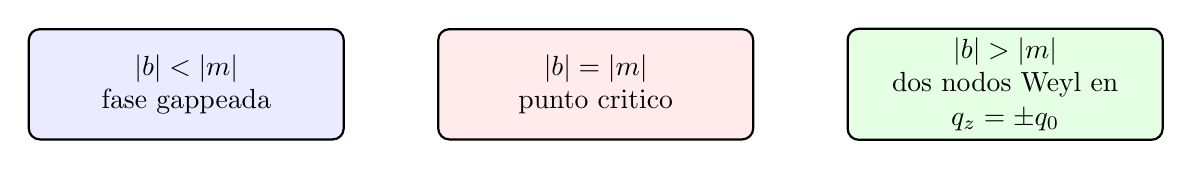
\begin{tikzpicture}[
    box/.style={draw, rounded corners, thick, align=center, minimum width=4cm, minimum height=1.4cm}
]
\node[box, fill=blue!8] at (0,0) {\(|b|<|m|\)\\fase gappeada};
\node[box, fill=red!8] at (5.2,0) {\(|b|=|m|\)\\punto critico};
\node[box, fill=green!10] at (10.4,0) {\(|b|>|m|\)\\dos nodos Weyl en\\\(q_z=\pm q_0\)};
\end{tikzpicture}
\caption{Secuencia conceptual: fase gappeada, punto critico y desdoblamiento en un par Weyl.}
\end{figure}

\section{Expansion alrededor de cada nodo}
Ahora tomamos
\begin{equation}
q_z = \pm q_0 + \delta q_z,
\qquad
q_x=\delta q_x,
\qquad
q_y=\delta q_y.
\end{equation}

Al expandir \eqref{c12:eq:lowspec} cerca de cada nodo se obtiene
\begin{equation}
E^2 \simeq
v^2(\delta q_x^2+\delta q_y^2)
+
v_z^2\,\delta q_z^2,
\end{equation}
con velocidad longitudinal
\begin{equation}
v_z = \frac{v^2 q_0}{|b|}
=
v\frac{\sqrt{b^2-m^2}}{|b|}.
\label{c12:eq:vz}
\end{equation}

Asi, cada nodo es un cono lineal anisotropo. El Hamiltoniano proyectado sobre el subespacio de baja energia toma la forma
\begin{equation}
H_\pm(\delta \bm{q})
\simeq
v\,\sigma_x \delta q_x
+
v\,\sigma_y \delta q_y
\pm
v_z\,\sigma_z \delta q_z.
\label{c12:eq:Weylpair}
\end{equation}

El signo \(\pm\) delante del termino longitudinal es justamente lo que hace que los dos nodos tengan quiralidad opuesta.

\subsection{Quiralidad}
La matriz de velocidades de \eqref{c12:eq:Weylpair} es
\begin{equation}
V_\pm = \mathrm{diag}(v,v,\pm v_z).
\end{equation}
Entonces
\begin{equation}
\chi_\pm = \mathrm{sign}\det V_\pm = \pm 1.
\end{equation}

Ya recuperamos exactamente el par Weyl esperado:
\begin{enumerate}[label=\arabic*.]
    \item dos nodos;
    \item separados en el espacio recíproco;
    \item con quiralidades opuestas.
\end{enumerate}

\section{Ahora la parte delicada: que pasa con los dobladores}
Todo lo anterior describe bien el sector ligero. Pero el paso realmente importante es demostrar que los dobladores pesados no se nos vuelven ligeros al encender \(b\).

\subsection{Masas de los distintos sectores}
En el capitulo anterior vimos que los distintos puntos especiales tienen masas efectivas
\begin{equation}
M_n = m + 2rN_n,
\qquad
N_n=0,1,2,3.
\label{c12:eq:Mn}
\end{equation}

Alrededor de cada uno de esos sectores, el Hamiltoniano efectivo tiene la misma estructura que \eqref{c12:eq:lightH}, pero con \(m\) reemplazado por \(M_n\). Por tanto el criterio de desdoblamiento en ese sector es
\begin{equation}
|b|>|M_n|.
\label{c12:eq:criterionMn}
\end{equation}

\subsection{Condicion para que solo se desdoble el sector central}
Queremos:
\begin{enumerate}[label=\arabic*.]
    \item que el sector central si se desdoble;
    \item que los otros no se desdoblen.
\end{enumerate}

Eso exige simultaneamente
\begin{equation}
|b|>|m|
\label{c12:eq:want1}
\end{equation}
y
\begin{equation}
|b|<
\min\left\{
|m+2r|,
|m+4r|,
|m+6r|
\right\}.
\label{c12:eq:want2}
\end{equation}

Estas dos desigualdades son la ventana de parametros verdaderamente importante del capitulo.

Si ademas estamos en el regimen del capitulo anterior,
\begin{equation}
|m|\ll 2r,
\end{equation}
entonces la condicion practica se vuelve muy clara:
\begin{equation}
\boxed{
|m|<|b|\ll 2r.
}
\label{c12:eq:mainwindow}
\end{equation}

\section{Interpretacion de la ventana \texorpdfstring{\(|m|<|b|\ll 2r\)}{|m|<|b|<<2r}}
Esta desigualdad resume todo el mecanismo.

\subsection{\texorpdfstring{Primer tramo: \(|b|>|m|\)}{Primer tramo: |b|>|m|}}
Garantiza que el Dirac ligero se rompa en dos Weyl.

\subsection{\texorpdfstring{Segundo tramo: \(|b|\ll 2r\)}{Segundo tramo: |b|<<2r}}
Garantiza que la perturbacion no sea lo bastante grande como para cerrar el gap de los dobladores asociados a masas \(m+2r\), \(m+4r\) y \(m+6r\).

\subsection{Consecuencia}
El resultado final es exactamente el que queriamos:
\begin{enumerate}[label=\arabic*.]
    \item un par Weyl aparece en el subsector central;
    \item los dobladores permanecen lejos en energia;
    \item la teoria infrarroja sigue estando limpia.
\end{enumerate}

\begin{figure}[h!]
\centering
\begin{tikzpicture}[
    box/.style={draw, rounded corners, thick, align=center, minimum width=4.1cm, minimum height=1.4cm},
    arr/.style={-{Latex[length=3mm]}, thick}
]
\node[box, fill=blue!8] (a) at (0,0) {\(|b|<|m|\)\\sector ligero gappeado};
\node[box, fill=yellow!10] (b) at (5.3,0) {\(|m|<|b|\ll 2r\)\\ventana buena};
\node[box, fill=red!8] (c) at (10.6,0) {\(|b|\sim 2r\) o mas\\dobladores en riesgo};
\draw[arr] (a) -- (b);
\draw[arr] (b) -- (c);
\end{tikzpicture}
\caption{La ventana de parametros que aisla un par Weyl controlado.}
\end{figure}

\section{Que hemos justificado realmente}
Vale la pena resumir con precision el alcance del argumento.

\subsection*{Lo que si demostramos}
\begin{enumerate}[label=\arabic*.]
    \item existe una perturbacion concreta que desdobla el sector Dirac ligero;
    \item el criterio del desdoblamiento es \(|b|>|m|\);
    \item los nodos aparecen en \(q_z=\pm q_0\);
    \item tienen quiralidad opuesta;
    \item si \(|m|<|b|\ll 2r\), los dobladores pesados no se activan.
\end{enumerate}

\subsection*{Lo que aun no hicimos}
Todavia no construimos una teoria completa de respuesta topologica o una derivacion formal de anomalias. Tampoco estudiamos aqui superficies de Fermi arco. Este capitulo se concentra solo en la pieza que realmente necesitabamos ahora:
\begin{displayquote}
\textbf{mostrar que el paso Dirac ligero \(\to\) par Weyl controlado puede hacerse sin perder el control infrarrojo del modelo.}
\end{displayquote}

\section{Conexion con el programa grande}
Este paso tiene mucha importancia dentro de la investigacion completa.

\subsection{Porque consolida la escalera conceptual}
Ahora la cadena ya no es solo cualitativa. Queda asi:
\begin{enumerate}[label=\arabic*.]
    \item red discreta;
    \item control de dobladores via Wilson;
    \item subsector Dirac ligero;
    \item desdoblamiento controlado a un par Weyl;
    \item estructura efectiva de quiralidad y grupos.
\end{enumerate}

\subsection{Porque protege la meta del proyecto}
Sin este paso, el lenguaje de Weyl podia quedarse en una intuicion local. Con este paso, ya tenemos una receta precisa para aislar el sector que se comporta de forma relativista y luego separar sus quiralidades sin que el resto de la red destruya el analisis.

\section{Mapa del siguiente paso}
Ahora tenemos dos caminos naturales y ambos son buenos:
\begin{enumerate}[label=\arabic*.]
    \item estudiar la estructura efectiva de simetria y los generadores en el par Weyl ya aislado;
    \item pasar a una lectura mas geometrica y topologica: curvatura de Berry, carga quiral y flujo entre nodos.
\end{enumerate}

\section{Resumen final}
Tomando el modelo de Wilson--Dirac ya depurado y agregando la perturbacion
\[
H_b = b\,\mathbb{I}_\tau\otimes \sigma_z,
\]
vimos paso a paso como el sector Dirac ligero puede desdoblarse en dos nodos Weyl separados a lo largo de \(k_z\). El criterio central es simple:
\[
|b|>|m|.
\]
En ese caso los nodos aparecen en
\[
q_z=\pm \frac{\sqrt{b^2-m^2}}{v},
\]
y su quiralidad es opuesta.

La parte realmente delicada era mostrar que esto puede hacerse sin volver a activar los dobladores pesados. Eso queda controlado por la ventana
\[
|m|<|b|\ll 2r,
\]
que garantiza que el sector central se desdobla mientras los sectores con masas \(m+2r\), \(m+4r\) y \(m+6r\) permanecen gappeados. Con eso ya tenemos un par Weyl infrarrojo limpio, surgido desde una red discreta bien controlada.
